\documentclass[12pt]{article} 
\usepackage[margin=1in]{geometry}
\usepackage{enumitem} %% for custom list
\usepackage{graphicx} %% for images
%\usepackage{multirow} %% for tables
%\usepackage{bigints}  %% for integrals
\usepackage{bytefield} %% for drawing packet structure
\usepackage{color} %% for color when drawing packet structure
\usepackage{array}

% used for tabbed spacing
%\newcommand{\itab}[1]{\hspace{0em}\rlap{#1}}
%\newcommand{\tab}[1]{\hspace{.4\textwidth}\rlap{#1}}

% using \code{come code monospaced}
\def\code#1{\texttt{#1}}

\begin{document}
\date{}
%\author{Andrea Ghizzoni \\
%some other info}
\title{\vspace{-11ex}} %% used for no title
 
\maketitle

\section{Livello Collegamento}\label{livello-collegamento}
Il livello Collegamento \textit{(o Data Link)} \'e l'ultimo strato del modello ISO/OSI prima che l'informazione venga 
trasmessa sul mezzo fisico. Si pu\'o definire come livello di \textit{"traduzione"} da un formato digitale ad uno 
elettrico dell'informazione.

Il problema principale deriva dal fatto che il livello collegamento dialoga direttamente con il mazzo trasmissivo, quindi 
deve sopperire a tutte le sue problematiche: molteplici tipi di mezzi trasmissivi ed errori derivanti dalle caratteristiche 
fisiche del mezzo. Questi errori sul canale vengono causati generalmente quando due o pi\'u segnali \textit{collidono} nel 
canale trasmissivo, ovvero sullo stesso canale due stazioni iniziano a trasmettere contemporaneamente, generando un segnale 
elettrico non pi\'u traducibile dal ricevitore in una sequenza digitale di bit. Questo problema prende il nome di 
\textbf{collision} \textit{(collisione)}.

Da un punto di vista implementativo il livello collegamento deve garantire lo stesso funzionamento sia attraverso onde radio 
che attraverso fibra ottica. Per permettere questa indipendenza dal mezzo trasmissivo effettivamente utilizzato \'e stato 
diviso logicamente in due parti sovrapposte: il vero livello collegamento, che ha principalmente funzione di controllo di 
flusso e incapsulamento, e il sottolivello \textbf{MAC} \textit{(Medium Access Control)}, che rende standard la 
comunicazione attraverso diversi mezzi trasmissivi.
\begin{center}
	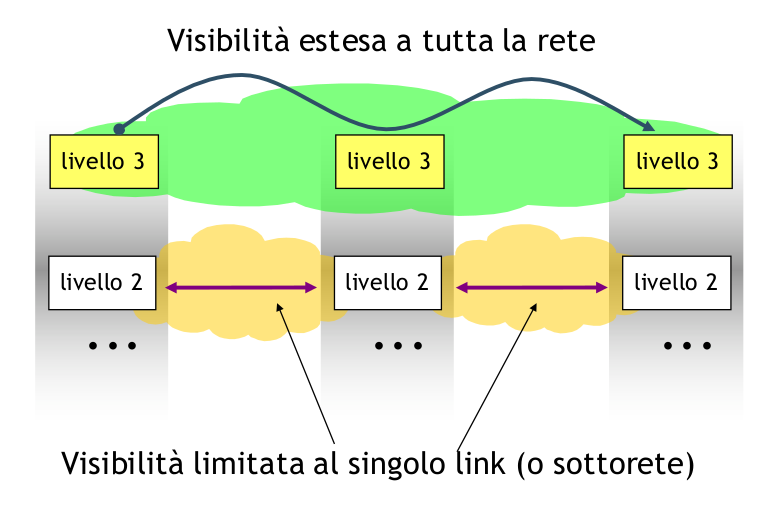
\includegraphics[scale=0.45]{livello_collegamento-img1.png}
\end{center}
A differenza dei livelli superiori, il livello collegamento \'e implementato direttamente nei firmware delle schede di rete  
invece che nel sistema operativo per motivi prestazionali: basti pensare che l'ordine di grandezza utilizzato a livello rete 
\'e in \code{ms} ($10^{-3}\ s$) invece a livello collegamento \'e \code{ns} ($10^{-9}\ s$), 

La visibili\'a del livello collegamento \'e limitata alle macchine adiacenti che condividono un mezzo fisico.

La PDU del livello collegamento viene definita \textbf{trama}.

\clearpage
\subsection{Funzioni}\label{livello-collegamento-funzioni}
Le funzioni del livello Collegamento sono dominate dal fatto che deve trasmettere le informazioni sul mezzo fisico, quindi:
\begin{itemize}
	\item \textbf{Framing}: delimitazione dei datagrammi in trame
	\item \textbf{Rilevazione degli Errori}: controllo di correttezza della trama
	\item \textbf{Controllo di Flusso}: regolazione della velocit\'a di invio in base al mezzo trasmissivo utilizzato
	\item \textbf{Controllo di Acceso al Canale}: regolazione dell'accesso al mezzo trasmissivo condiviso
\end{itemize}

\subsubsection{Framing}\label{livello-collegamento-funzioni-framing}
Con \textbf{Framing} \textit{(Suddivisione)} si identificano tutte quelle tecniche che delimitato delle informazioni 
digitali per la trasmissione su un mezzo elettrico. Questa necessit\'a nasce dal fatto che il livello fisico sottostante 
tratta solo bit e non \'e in grado di distinguere dove inizia un datagramma e il successivo.

Bisogna considerare inoltre che questi sistemi sono fortemente influenzati dalla temporizzazione e dalla sincronizzazione
dei segnali, quindi un'ulteriore compito del livello collegamento \'e quello di creare un meccanismo di 
\textbf{sincronizzazione} della trama.

La funzionalit\'a di framing dunque rendere distinguibile una trama dall'altra attraverso l'utilizzo di \textbf{header} 
\textit{(intestazione)} all'inizio e di \textbf{trailer} \textit{(finale)} alla fine della trama stessa.
\begin{center}
	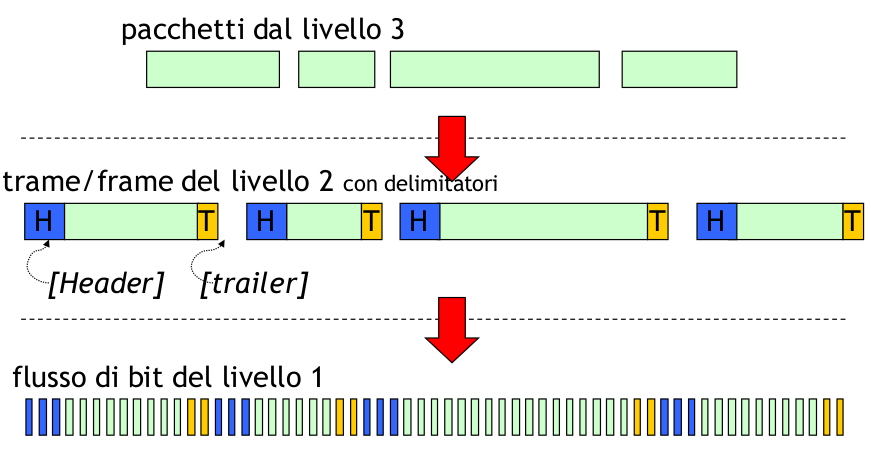
\includegraphics[scale=0.35]{livello_collegamento-img2.png}
\end{center}
La tecnica pi\'u ovvia per delimitare le trame sarebbe quella di inserire degli intervalli temporali tra trame consecutive; 
ma questo approccio, a causa della natura intrinseca delle reti di comunicazione, ovvero che non possono garantire le 
caratteristiche temporali delle informazioni trasmesse, gli intervalli potrebbero essere espansi o ridotti generando 
problemi in ricezione.

La tecnica effettivamente utilizzata \'e quella di inserire, per ogni trama dei \textbf{codici di controllo}.

\paragraph{Character Count} In questo caso l'header consiste nel numero di byte che la trama contiene. Come \'e
facilmente immaginabile non \'e l'approccio pi\'u sicuro, in quanto se, per qualche motivo, il numero di byte nell'header
viene modificato, il ricevente ne legger\'a un numero non valido, andando fuori sincronica.

\paragraph{Bit Stuffing} Questa tecnica parte dall'idea di utilizzare i dati stessi come delimitatori attraverso l'euristica
dei 5 \textit{"1"}: quando il trasmettitore deve inviare una sequenza di cinque bit impostati a "1" ne inserisce uno "0" 
subito dopo, quindi in ricezione verr\'a eseguito il processo inverso, ripristinando il flusso di dati originale.

\paragraph{Byte Stuffing} Il Byte Stuffing era la tecnica utilizzata dalla telescriventi. Utilizzando un sistema di 
comunicazione a caratteri \'e naturale pensare che si riservino dei caratteri \textit{speciali} per delimitare le trame:
\begin{itemize}[noitemsep]
	\item \code{DLE} \textit{(Data Link Escape)} + \code{STX} \textit{(Start of TeXt)} come header
	\item \code{DLE} \textit{(Data Link Escape)} + \code{ETX} \textit{(End of TeXt)} come trailer
\end{itemize}
Come si pu\'o facilmente osservare la sorgente duplica il carattere DLE.

\paragraph{Violazione di Codifica} Quest'ultima tecnica utilizza fortemente le caratteristiche di trasmissione del 
livello fisico. Infatti nel livello sottostante abbiamo una mappatura di ogni bit con un livello di tensione "alto" o
"basso". Se si assume che ogni bit viene invece mappato con una coppia di questi livelli di tensione, si possono 
identificare delle coppie non valide, quindi utilizzabili come inizio/fine trama.

\textbf{Esempio:} "1" mappato con "AB", mentre "0" mappato con "BA". Se nel flusso di byte si trovano sequenze del tipo "AA" 
o "BB" riconosco che \'e un inizio o fine trama.

\subsubsection{Rilevamento e Correzione degli Errori}\label{livello-collegamento-funzioni-rilevamento-errori}
Essendo che il livello collegamento riceve i dati direttamente dal mezzo fisico, purtroppo sono pieni di errori sotto forma 
di distorsioni, attenuazioni ed errori nei dati. Lo strato pi\'u alto del livello collegamento prevede l'incapsulamento 
dell'informazione per aggiungere ad ogni trama un campo \textbf{Checksum}, che funge da meccanismo di controllo della
correttezza.

\subsubsection{Controllo di Flusso}\label{livello-collegamento-funzioni-controllo-di-flusso}
Data il fatto che il livello collegamento non deve consegnare i dati alle applicazioni (generalmente molto lente nel 
leggerli) ma  deve occuparsi della ricostruzione e la consegna al livello di rete, generalmente ha il controllo completo del 
mezzo trasmissivo. Pu\'o succedere che la sorgente vuole trasmettere delle trame pi\'u velocemente di quanto la destinazione 
sia in grado di gestirli. Per evitare questo problema esistono due metodi di controllo di flusso bastati su:
\begin{itemize}[noitemsep]
	\item \textbf{feedback}: la sorgente in Stop\&Wait invia i dati e aspetta un riscontro dalla destinazione
	\item \textbf{tasso di invio}: il protocollo della sorgente \'e progettato ad-hoc per la rete sottostante, quindi 
	      pu\'o gestire il tasso di invio in modo efficiente; unico svantaggio \'e che servono moltissimi protocolli di 
	      questo tipo
\end{itemize}



\clearpage
\section{Il Sotto-livello MAC}\label{mac}
Essendo che il livello collegamento utilizza direttamente il mezzo trasmissivo, \'e necessario che si adatti ad ogni sua 
caratteristica; basti pensare alle differenze fisiche di un collegamento tramite onde elettromagnetiche nell'aria e tramite 
impulsi luminosi nelle fibre ottiche.

Ma la natura fisica del canale non basta, bisogna tenere conto che un mezzo trasmissivo pu\'o essere condiviso 
contemporaneamente tra pi\'u stazioni, chiamate reti \textbf{broadcast} \textit{(multi-punto)}, oppure pu\'o collegare 
direttamente la sorgente con la destinazione, reti \textbf{point-to-point} \textit{(punto-a-punto)}. Per far fronte a queste 
problematiche \'e necessario che vengano implementate delle tecniche di \textbf{accesso al canale}, in modo tale da 
minimizzare le collisioni e massimizzare la velocit\'a di trasmissione per ogni stazione.

Per questi motivi, \'e stato diviso logicamente il livello collegamento in due \textit{parti} sovrapposte: il livello 
collegamento e il \textbf{sotto-livello MAC} \textit{(Mediumn Access Controll)}; dove \'e stato previsto che comunicasse 
direttamente con il livello Fisico sottostante, per risolvere il problema dell'accesso al canale.

Il sotto-livello MAC quindi, implementa tutte le caratteristiche di ogni possibile classe di mezzo trasmissivo: quindi ci 
sar\'a il sotto-livello MAC dedicato alla trasmissione tramite onde radio (WiFi) o tramite mezzo in rame (Ethernet).
\begin{center}
	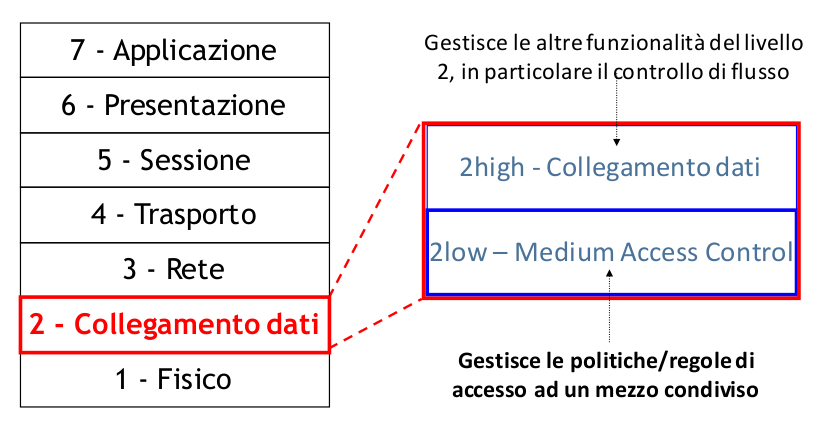
\includegraphics[scale=0.45]{livello_collegamento-img3.png}
\end{center}
Si pu\'o quindi dire che non \'e indipendente dal livello Fisico sottostante; una chiara violazione dell'indipendenza degli 
strati protocollari di ISO/OSI.

\clearpage
\subsection{Allocazione del Canale}\label{mac-allorazione-canale}
Il problema principale che il sottolivello MAC deve risolvere \'e l'accesso concorrenziale al mezzo trasmissivo, ovvero 
gestire tutte quelle situazione in cui il canale trasmissivo \'e unico ed \'e condiviso da parte di pi\'u sorgenti.

\subsubsection{Allocazione Statica}
La condivisione di un mezzo trasmissivo pu\'o essere risolta facilmente assegnando staticamente una \textit{"quota"} di 
capacit\'a trasmissiva a ciascuna delle stazioni, dove per quota si intende:
\begin{itemize}[noitemsep]
	\item tempo: ogni stazione ha a disposizione tutto il canale trasmissivo per un determinato intervallo di tempo
	\item frequenza: ad ogni stazione \'e assegnata una frequenza di trasmissione, ovvero una determinata banda\footnote{Da 
	      notare che le stazioni radio FM utilizzano il principio di allocazione del canale a divisione di frequenza.}
\end{itemize}
Questa tecnica di allocazione pu\'o risultare semplice e conveniente quando al mezzo trasmissivo sono collegati solo pochi 
utenti con molti dati da trasmettere e/o ricevere. Nel momento in cui in questa situazione il numero di utenti cresce, 
nessuno riuscir\'a pi\'u ne a trasmettere ne a ricevere, perch\'e non ha a disposizione una quota sufficiente di utilizzo del 
canale che che gli permetta di massimizzare l'utilizzo del mezzo. In aggiunta: se a una stazione che non ha nulla da 
trasmettere e gli viene assegnato l'utilizzo esclusivo del canale, la capacit\'a di trasmissione verr\'a sprecata.

\subsubsection{Allocazione Dinamica} \label{mac-allorazione-canale-dinamica}
Ovviamente in questa categoria rientrano tutte le tecniche di allocazione del mezzo trasmissivo che non richiedono una 
qualche divisione in quote dello stesso. Possiamo individuare due famiglie di tecniche di allocazione del canale:
\begin{itemize}[noitemsep]
	\item a turno:  viene trasmesso \textit{"permesso"} di trasmettere (reti \textit{Token Ring})
	\item a contesa: tutte le stazioni sono indipendenti dalle altre e sono in continua competizione per l'uso del 
		  canale
\end{itemize}
La prima famiglia porta tutta una serie di problemi quali: l'assegnazione del permesso a trasmettere, la durata e come questo 
deve essere condiviso alla fine della trasmissione.

La famiglia delle tecniche a contesa, invece, non risente di particolari problemi in quanto, in un certo senso, non ci sono
meccanismi di allocazione: ogni stazione che desidera trasmettere sul canale \'e libera di farlo, controllando che nessun 
altro lo stia usando.

\clearpage
\subsection{Allocazione del canale a Contesa}\label{mac-allorazione-canale-a-contesa}
La tecnica utilizzata nel sottolivello MAC \'e basata sull'allocazione dinamica a contesa. Per permettere l'analisi analitica 
di questa classe di protocolli sono necessarie i seguenti presupposti:
\begin{itemize}[]
	\item \textbf{Canale Singolo}: esiste un solo canale usato per tutto il tempo della comunicazione che pu\'o essere 
	      condiviso tra pi\'u stazioni
	\item \textbf{Stazioni Indipendenti}: $N$ stazioni sul tratto di rete indipendenti l'una dalle altre nell'invio di trame 
	      di livello collegamento. Le trame sono generate secondo una distribuzione di Poisson con media $G$. 
	      La lunghezza della trama \'e fissa, ovvero il tempo di trasmissione \'e costante e pari a $T$, chiamato anche tempo 
	      di trama.
	\item \textbf{Collisioni Osservabili}: tutte le stazioni sono in grado di rilevare una collisione sul canale. Non sono 
	       presenti altre forme di errore
	\item \textbf{Tempo}: vengono usati due metriche per contare il tempo:
	      \begin{itemize}[noitemsep]
				\item continuo: una trama pu\'o essere inviata in qualsiasi momento
				\item slotted: una trama pu\'o essere inviata solo in istanti discreti
		  \end{itemize}
	\item \textbf{Rilevamento della Portante}: ogni stazione deve essere in grado di percepire il segnale portante di un 
	      canale per capire se un'altra stazione sta trasmettendo
\end{itemize}

\clearpage
\subsubsection{ALOHA Puro} \label{mac-allorazione-canale-a-contesa-aloha-puro}
Il primo meccanismo a livello MAC \'e stato introdotto negli anni '70 per permettere ad alcune 
stazioni radio dell'Universit\'a delle Hawaii di scambiarsi informazioni.

Nella versione di Aloha Puro prevede che ogni stazione possa trasmettere in ogni istante di tempo, se viene generata una 
collisione, la destinazione non inviar\'a un riscontro quindi la sorgente aspetter\'a un tempo casuale prima di 
ritentare la trasmissione. L'idea dell'attesa di un tempo casuale \'e dovuta al fatto che un'attesa di un tempo 
deterministico potrebbe portare a collisioni all'infinito.

Questo significa che per ogni tempo di trama $T$ che inizia la trasmissione all'istante $t_0$ non devono iniziare altre
trasmissioni nel tempo $t_0-T$ e $t_0+T$, quindi per un tempo di $2T$; questo viene definito come \textbf{periodo di 
vulnerabilit\'a}, ovvero il tempo nel quale possono accadere delle collisioni.
\begin{center}
	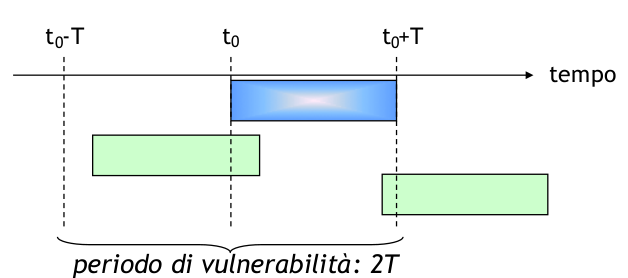
\includegraphics[scale=0.49]{livello_collegamento-img4.png}
\end{center}
Di conseguenza si pu\'o definire il throughput, ovvero numero medio di trame trasmesse del protocollo $S$ in termini di 
traffico generato $G$:
\begin{center}
	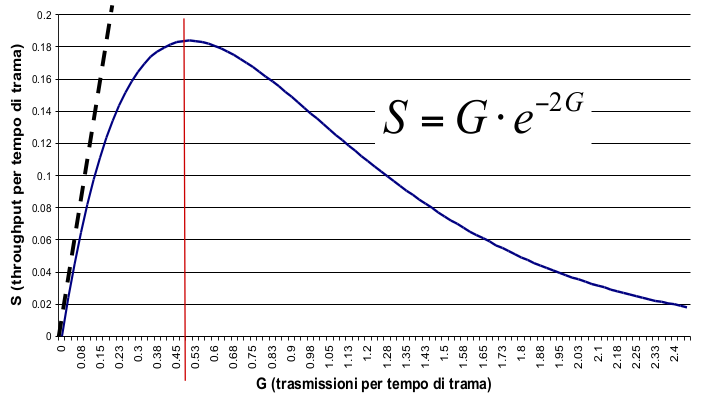
\includegraphics[scale=0.6]{livello_collegamento-img5.png}
\end{center}
Come si nota dalla distribuzione, Aloha Puro permette di sfruttare il 19\% del tempo di trama quando il traffico
offerto \'e $\approx 0.5$ volte la capacit\'a del canale; quindi e' un protocollo altamente \textbf{instabile}.

\clearpage
\subsubsection{ALOHA Slotted}\label{mac-allorazione-canale-a-contesa-aloha-slotted}
Una miglioria apportata al protocollo Aloha Puro \'e stata quella di usare un tempo discreto 
per l'inizio della trasmissione di ogni trama, in questo modo ogni stazione pu\'o iniziare a trasmettere solo in un 
preciso istante di tempo $t_0$. 

Il diretto vantaggio di questa semplice migliorai \'e il dimezzamento del periodo di vulnerabilit\'a al costo di creare un 
sistema di distribuzione e mantenimento del sincronismo tra le stazioni.
\begin{center}
	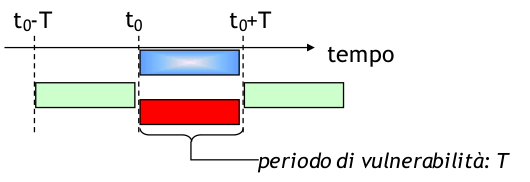
\includegraphics[scale=0.65]{livello_collegamento-img6.png}
\end{center}
Le prestazioni dello Slotted Aloha non sono molto diversi da Aloha Puro ma vengono migliorati alcuni aspetti.
\begin{center}
	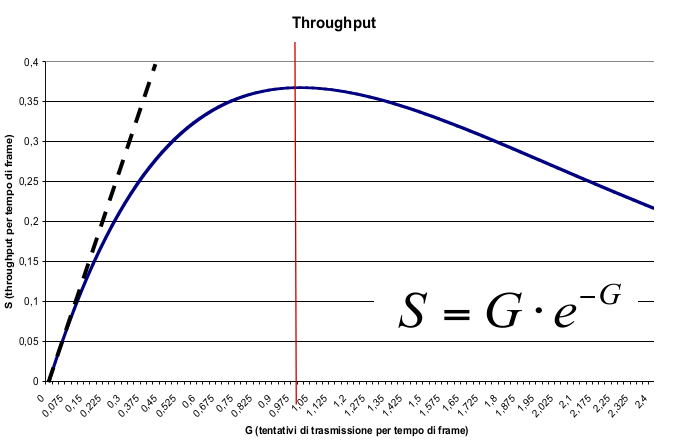
\includegraphics[scale=0.6]{livello_collegamento-img7.png}
\end{center}
Slotted Aloha utilizza il 37\% dei tempi di trama e avviene solo quando il traffico offerto \'e circa parti alla capacit\'a 
del canale. Come Aloha Puro \'e ancora un protocollo instabile.

\clearpage
\subsubsection{Carrier Sense Multiple Access}\label{mac-allorazione-canale-a-contesa-csma}
Un'altra tecnica per gestire l'accesso multiplo al mezzo trasmissivo \'e quello di \textit{"ascoltare"} la portante del 
canale per capire se altre stazioni stanno trasmettendo: se il canale \'e libero, la stazione trasmette sena problemi, 
altrimenti sono possibili le seguenti varianti:
\begin{itemize}
    \item \textbf{CSMA-1-persistente}: quando una stazione deve trasmettere, prima controlla che il canale sia libero e 
          privo di collisioni, poi inizia a trasmettere. Se trova il canale occupato, la stazione aspetta finch\'e non si 
          libera. Il protocollo viene detto "1-persistente" perch\'e trasmette con probabilit\'a 1 quando il canale \'e     
          libero.
    \item \textbf{CSMA-0-persistente}: questo protocollo \'e equivalente a CSMA-1-persistente ma invece di continuare ad 
          ascoltare il canale nel caso di una collisione per impossessarsene il prima possibile, aspetta un tempo casuale 
          molto pi\'u grande del tempo di trama prima di effettuare di nuovo il controllo. Questo garantisce una migliore 
          allocazione del canale ma allunga il ritardo rispetto a CSMA-1-persistente.
    \item \textbf{CSMA-p-persistente}: si applica a canali divisi in intervalli di tempo. Quando una stazione \'e pronta 
          a trasmettere e trova il canale libero, trasmette subito con probabilit\'a $p$ e rimanda la trasmissione con 
          probabilit\'a $1-p$.
\end{itemize}
Nel seguente grafico vengono rappresentate tutte le tecniche presentate fino ad ora:
\begin{center}
	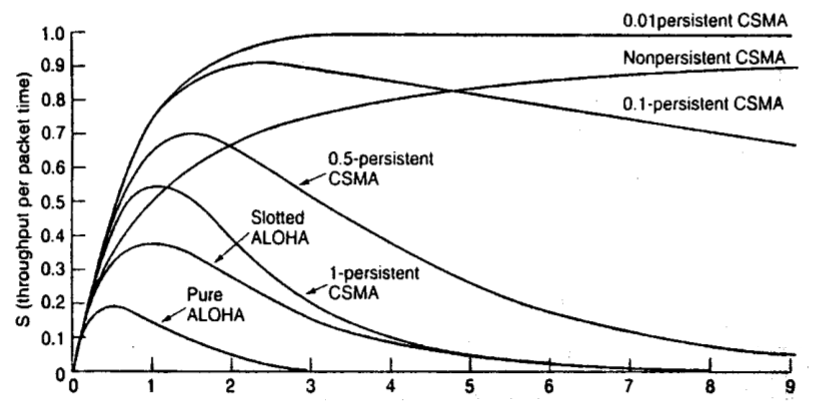
\includegraphics[scale=0.6]{livello_collegamento-img8.png}
\end{center}

\clearpage
\subsubsection{Carrier Sense Multiple Access with Collision Detection}\label{mac-allorazione-canale-a-contesa-csma-cd}
CSMA porta un notevole miglioramento rispetto ad Aloha, ma esiste ancora il seguente problema: se due stazioni rilevano il 
canale libero allora inizieranno la trasmissione, causando inevitabilmente una collisione. Se la stazione fosse in grado
di rilevare una collisione mentre sta trasmettendo, sarebbe in grado di terminare bruscamente la comunicazione e mettersi
in attesa che il canale si liberi.

Questa tecnica prende il come di CSMA-CD \textit{(Carrier Sense Multiple Access with Collision Detection)} ed \'e pi\'u
efficiente delle precedenti perch\'e non spreca tempo a trasmettere trame gi\'a corrotte o che andranno corrotte finch\'e 
il canale non si libera.

Ovviamente CSMA-CD pu\'o essere usato solo in reti cablate, in quanto in reti wireless \'e sostanzialmente impossibile 
rilevare un segnale aggiuntivo rispetto a quello trasmesso.

In caso di collisione, CSMA-CD applica la tecnica chiamata \textbf{binary exponential backoff}, ovvero dopo $i$ collisioni
l'host attende prima di ri-iniziare la procedura di trasmissione un tempo casuale nell'intervallo $[0,1,...,2^i-1]$. 
Ovviamente se $10 \leq i < 16$ collisioni l'intervallo \'e limitato a $[0,1,...,1023]$, mentre se $i \geq 16$ viene 
riportato al sistema operativo un errore di rete.

Nell'immagine seguente si vede in rosso in throughput del protocollo CSMA-CD con binary esponential backoff:
\begin{center}
	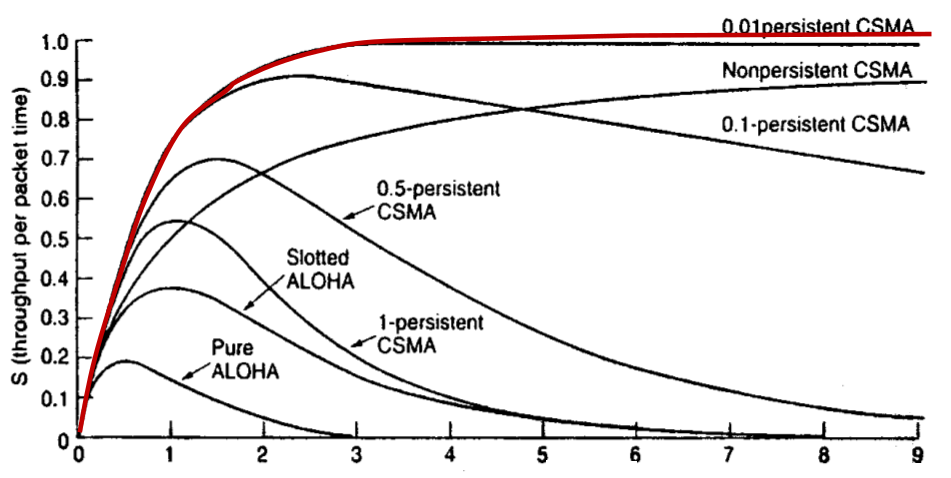
\includegraphics[scale=0.5]{livello_collegamento-img9.png}
\end{center}

\clearpage
\subsubsection{Riassunto}\label{mac-allorazione-canale-a-contesa-riassunto}
\begin{center}
	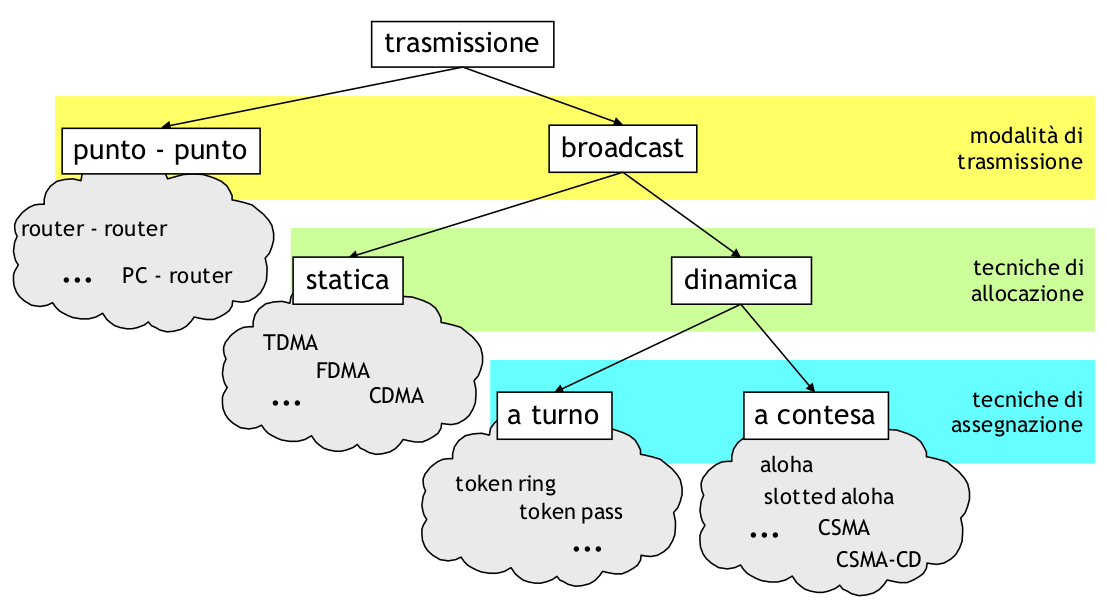
\includegraphics[scale=0.4]{livello_collegamento-img15.png}
\end{center}



\clearpage
\section{Standard IEEE 802}\label{ieee-802}
Il livello collegamento \'e stato completamente definito dallo standard IEEE 802, numero che indica semplicemente la data di 
standardizzazione 8 febbraio 1980, che comprende:
\begin{itemize}[noitemsep]
	\item 802.1: LAN \textit{internetworking}
	\item 802.2: LLC
	\item 802.3: CSMA/CD in Ethernet
	\item 802.4: Token Bus
	\item 802.5: Token Ring 
	\item 802.6: DQDB per MAN
	\item 802.7: Broadband Technical Advisor Group
	\item 802.8: Fiber-Optic Techincal Advisor Group
	\item 802.9: Integrated Data and Voice Networks
	\item 802.10: Network Security
	\item 802.11: Wireles Network (/a/b/g/h/f/s/n/p/ac/...)
	\item 802.12: 100base VG
	\item 802.13: 100base X
	\item 802.15: Personal Area Network (bluetooth...)
	\item 802.16: Wireless MAN
\end{itemize}
\'E necessario notare che \'e stato aggiunto un ulteriore strato comune a tutti i livelli MAC: \textbf{LLC} \textit{(Logical 
Link Controll)}, con la funzione di standardizzare il formato delle trame attraverso tutti i protocolli MAC esistenti. Il 
sottolivello LLC \'e indipendente dal livello fisico, cosa non vera per il livello MAC.
\begin{center}
	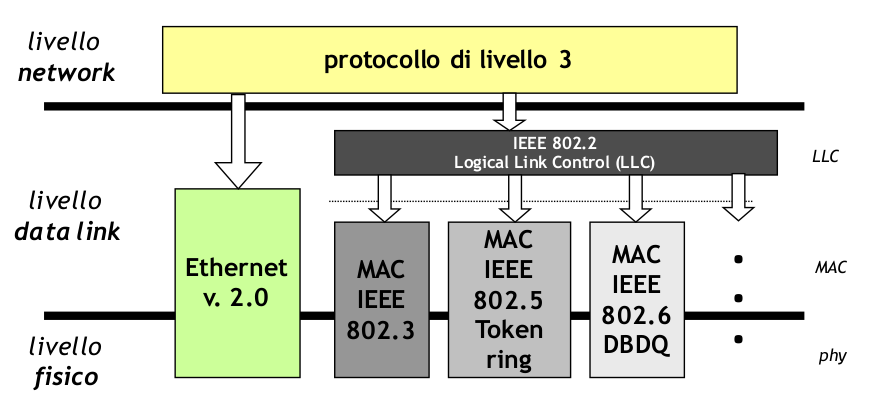
\includegraphics[scale=0.4]{livello_collegamento-img16.png}
\end{center}
Come si nota dalla figura, la prima implementazione di Ethernet non prevedeva il sottolivello LLC.

\clearpage
\subsection{Formato della Trama Ethernet in 802.3}\label{ieee-802-formato-trama-ethernet-802.3}
Il formato della trama Etherenet nel sottolivello MAC \'e cos\'i composta:\\
\begin{center}
\begin{bytefield}[bitwidth=1em]{32}
	\bitheader{0,7,8,15,16,23,24,31}\\
	\begin{rightwordgroup}{header\\24 byte}	
		\bitbox[ltr]{32}{Preambolo}\\ 
		\bitbox[lrb]{24}{} & \bitbox[lrtb]{8}{Inizio Frame}\\ 
		\bitbox[ltr]{32}{MAC Sorgente}\\ 
		\bitbox[lrb]{24}{} & \bitbox[t]{8}{}\\
		\bitbox[ltr]{32}{MAC Destinazione}\\ 
		\bitbox[lrb]{24}{} & \bitbox[t]{8}{}\\
		\bitbox{16}{Lunghezza}
	\end{rightwordgroup}\\
	\begin{rightwordgroup}{payload\\46-1500\\byte}	
		\wordbox{5}{Dati}		
	\end{rightwordgroup}\\
	\bitbox{32}{Checksum}\\
	\wordbox{3}{Inter Frame Gap}
\end{bytefield}
\end{center}
\textbf{NB}: la scala in alto \'e in byte.\\
\begin{itemize}
	\item \textbf{Preambolo}: sequenza utilizzata per sincronizzare il ricevitore
	\item \textbf{Inizio Frame}: flag di inizio trama per separarla dal preambolo
	\item \textbf{MAC Sorgente/Destinazione}: indirizzo MAC sorgente e destinazione
	\item \textbf{Lunghezza}: lunghezza in byte della trama (max 1500 byte), se maggiore di 1500 indica il tipo di protocollo 
	      usato
	\item \textbf{Dati}: informazione da trasmettere dei livelli superiori
	\item \textbf{Checksum}: codice di controllo
	\item \textbf{Inter-Frame-Gap}: tempo di bit per permettere al ricevitore di prepararsi alla ricezione della prossima 
	      trama
\end{itemize}

\clearpage
\subsection{Il livello Fisico in Ethernet 802.3}\label{ieee-802-livello-fisico-in-802.3}
Il numero davanti a BASE indica la velocit\'a in Mbps:
\subsubsection{Ethernet}\label{ieee-802-livello-fisico-in-802.3-ethernet}
\begin{tabular}{ m{4cm} | m{3cm} | c | m{5cm}}
    \textbf{Nome} & \textbf{Cavo} & \textbf{Lunghezza Max} & \textbf{Vantaggi} \\[2pt]\hline
    10 BASE 5 & Coassiale Spesso & 500 m & Prima implementazione \\[2pt]\hline
    10 BASE 2 & Coassiale Sottile & 185 m & Usa la stessa configurazione di 10 BASE 5 \\[2pt]\hline
\end{tabular}
\subsubsection{Fast Ethernet}\label{ieee-802-livello-fisico-in-802.3-fast-ethernet}
\begin{tabular}{ m{4cm} | m{3cm} | c | m{5cm}}
    \textbf{Nome} & \textbf{Cavo} & \textbf{Lunghezza Max} & \textbf{Vantaggi} \\[2pt]\hline
    100 BASE-T4 & Doppino UTP & 100 m & Adatto a cablaggi strutturati. Usato per collegare le stazioni agli Hub\\[2pt]\hline
    100 BASE-TX & Doppino UTP & 100 m & come 100 BASE-T4 ma Full Duplex \\[2pt]\hline
    100 BASE-FX & Fibra & 2 Km & Aumenta la distanza \\[2pt]\hline
\end{tabular}
\subsubsection{Gigabit Ethernet}\label{ieee-802-livello-fisico-in-802.3-gigabit-ethernet}
\begin{tabular}{ m{4cm} | m{3cm} | c | m{5cm}}
    \textbf{Nome} & \textbf{Cavo} & \textbf{Lunghezza Max} & \textbf{Vantaggi} \\[2pt]\hline
    1000 BASE-SX & Fibra & 550 m & Utilizzo di Fibra Multimodale \\[2pt]\hline
    1000 BASE-LX & Fibra & 5 Km & Utilizzo di Fibra Multi o Monomodale\\[2pt]\hline
    1000 BASE-CX & 2 coppie STP & 25 m & Uso di doppino schermato\\[2pt]\hline
    1000 BASE-T & 4 coppie UTP & 100 m & UDP cat.5\\[2pt]\hline
\end{tabular}
\subsubsection{10-Gigabit Ethernet}\label{ieee-802-livello-fisico-in-802.3-10gigabit-ethernet}
\begin{tabular}{ m{4cm} | m{3cm} | c | m{5cm}}
    \textbf{Nome} & \textbf{Cavo} & \textbf{Lunghezza Max} & \textbf{Vantaggi} \\[2pt]\hline
    10G BASE-SR & Fibra & 300 m & Utilizzo di Fibra Multimodale \\[2pt]\hline
    10G BASE-LR & Fibra & 10 Km & Utilizzo di Fibra Monomodale\\[2pt]\hline
    10G BASE-ER & Fibra & 40 Km & Utilizzo di Fibra Monomodale\\[2pt]\hline
    10G BASE-CX4 & 4 coppie biassiali & 15 m & Rame Biassiale \\[2pt]\hline
    10G BASE-T & 4 coppie UTP & 100 m & UTP cat.6 \\[2pt]\hline
\end{tabular}

\clearpage
\subsection{Evoluzione di Ethernet}\label{ieee-802-evoluzione-di-ethernet}
Il progetto originale di Ethernet prevedeva un lungo cavo coassiale, chiamato \textbf{Thick Ethernet}, che serviva per 
collegare tutte le stazioni della rete. 
\begin{center}
	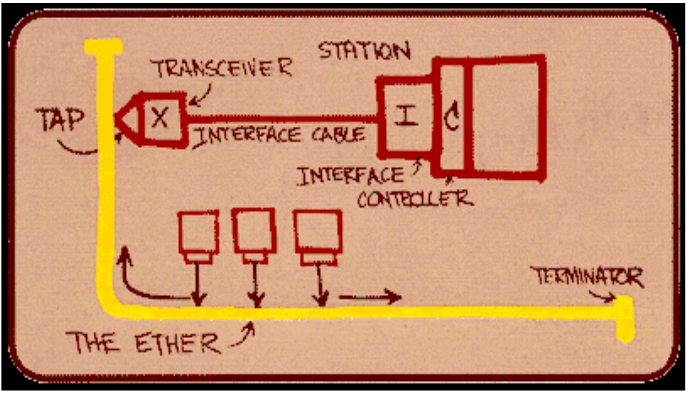
\includegraphics[scale=0.5]{livello_collegamento-img10.png}
\end{center}
Per poter permettere alle stazioni di usare il cavo, era previsto un \textbf{Transceiver}, ovvero un meccanismo ad uncino che 
andava a forare il cavo coassiale e toccava il cavo metallico all'interno e la calza esterna dello stesso, in questo modo si 
creava una derivazione verso stazione.

Ovviamente forare il mezzo trasmissivo per aggiungere una stazione non \'e sostenibile a lungo termine, infatti ne 
risentivano le misure massime di cavo che si potevano utilizzare: la lunghezza massima del cavo coassiale era di 500 m con un 
massimo di 100 stazioni, la lunghezza del cavo del transceiver era di 50 m e non ci potevano essere pi\'u di 5 ripetitori tra 
due stazioni. La velocit\'a massima raggiungibile con questa configurazione era di 10 Mbps.

Presto la configurazione a singolo cavo condiviso tra le stazioni venne abbandonato a favore di una configurazione di 
pi\'u facile gestione: ogni stazione veniva collegata, con il proprio cavo, ad un \textbf{Hub} centrale, il quale fungeva da 
"canale" condiviso.

Con il crescere del traffico e del numero di stazioni, gli hub divennero spesso coni di bottiglia per la rete: sostituendolo
con uno \textbf{Switch} si risolvono questi problemi.
\begin{center}
	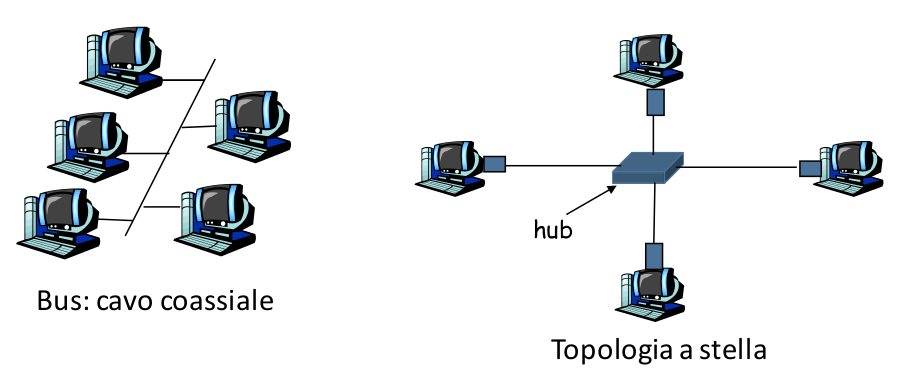
\includegraphics[scale=0.4]{livello_collegamento-img11.png}
\end{center}

\paragraph{Dominio di Collisione} Si definisce \textit{Dominio di Collisione} quella porzione di rete Ethernet in cui, se 
due stazioni trasmettono simultaneamente, le trame collidono.

\paragraph{Dominio di Broadcast} Si definisce \textit{Dominio di Broadcast} quella parte di rete raggiunta da una segmento di 
livello rete con indirizzo broadcast. Diversi domini di broadcast devono essere separati da un router.
\begin{center}
	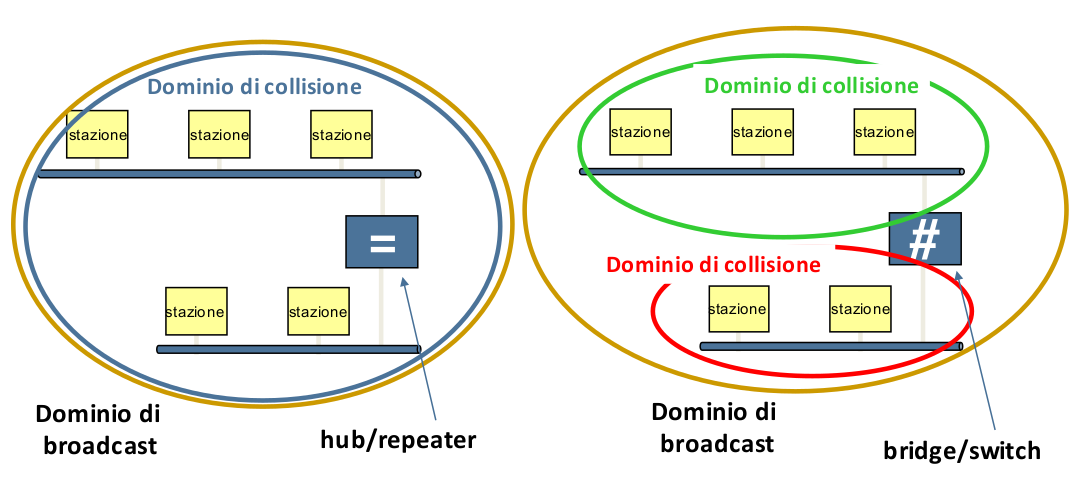
\includegraphics[scale=0.4]{livello_collegamento-img12.png}
\end{center}

\subsection{Repeater e Hub}\label{ieee-802-repeater-hub}
Originariamente vennero impiegati i dispositivi chiamati \textit{Hub} o \textit{Repeater}, per non usare un unico cavo
coassiale come mezzo di comunicazione condiviso.

Un hub lavora direttamente sulle trame di livello fisico, replicandole in \textbf{flooding} ogni segnale da una linea in
tutte le altre, ed eventualmente amplificandolo.
\begin{center}
	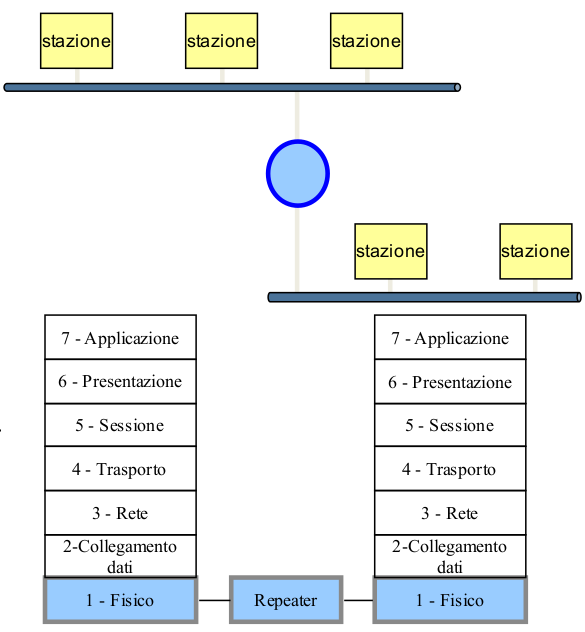
\includegraphics[scale=0.35]{livello_collegamento-img13.png}
\end{center}
Il problema di questo tipo di rete \'e che estendono molto il dominio di collisione.


\subsection{Bridge e Switch}\label{ieee-802-bridge-switch}
L'apparato di rete \textit{Bridge} sopperisce ai problemi di cui soffriva l'hub: il bridge collega due segmenti di rete
spezzandone il dominio di collisione. 

Per riuscire in questo non si deve limitare a ritrasmettere le trame di livello fisico a tutti i segmenti di rete collegati, 
ma deve riconoscere a quale segmento di rete inoltrare le trame.
\begin{center}
	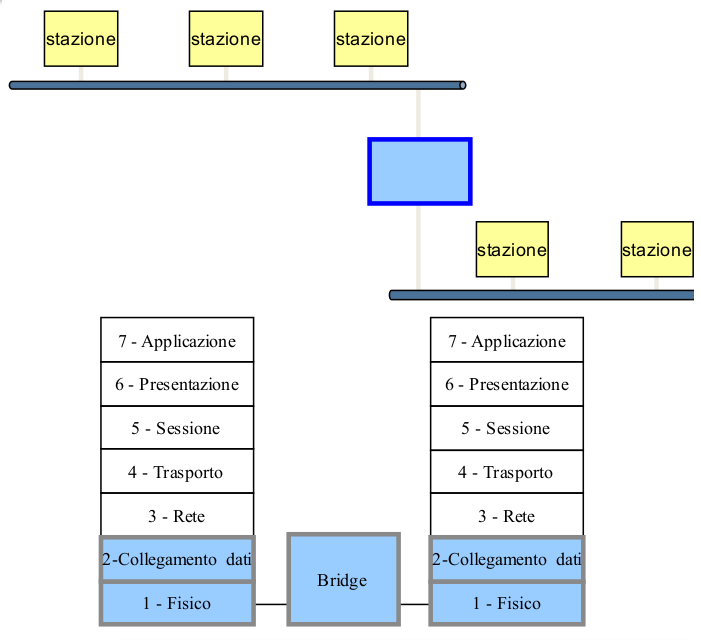
\includegraphics[scale=0.35]{livello_collegamento-img14.png}
\end{center}
I bridge applicano le tecniche di \textbf{Store and Forward} per decidere se inoltrarlo all'altro segmento di rete, oppure 
sullo stesso di ricezione.

Questi apparati di rete agiscono come porte tagliafuoco, impedendo ad una stazione impazzita di compromettere le 
prestazioni dell'intera rete. Perch\'e questo accada il bridge deve essere completamente trasparente a livello utente, motivo 
per il qualche lavora a livello collegamento.

L'evoluzione dei bridge sono i \textbf{Layer 2 Switch} o comunemente chiamati \textbf{Switch}. Gli switch sono dei bridge
multiporta.

\subsubsection{Backword Learning} \label{ieee-802-backward-learning}
L'algoritmo utilizzato dagli switch per decidere su che porte inoltrare il frame di livello collegamento si chiama 
\textbf{Backword Learning} \textit{(Apprendimento Rovescio)}, e consiste nel tenere una tabella hash con la coppia 
destinazione-porta- in modo tale da leggere l'indirizzo MAC di destinazione di ogni frame e indirizzarlo sulla porta giusta.

Questo algoritmo ha una fase di inizializzazione quando la tabella \'e vuota: in questo caso ogni frame viene fatto uscire 
su tutte le porte, eccetto quella di entrata, e col passare del tempo lo switch impara (riempie la tabella) dove sono le
stazioni (da che porta proviene la risposta a quel frame).

Per gestire i cambiamenti della topologia dinamicamente, viene inserito nella tabella un campo per segnare il tempo di 
arrivo dell'ultimo frame per ogni porta; in questo modo un processo pu\'o pulire la tabella delle entry vecchie e non pi\'u 
raggiungibili.

\subsubsection{Virtual LAN} \label{ieee-802-vlan}
Una necessit\'a \'e di separare le LAN in modo da bilanciare il traffico e venire in contro alle singole esigenze delle LAN.

La risposta ad una maggiore flessibilit\'a \'e la \textit{VLAN} o (\textit{Virtual-LAN}), che permette di separare il 
dominio di collisione all'interno dello switch stesso via software. Per realizzare questo tipo di archittettura \'e 
necessario uno switch particolare che permetta di creare VLAN.

\end{document}